% Section: clist (\input from main.tex)
\section{The Concurrent Set Data Structure}
\label{sec:clist}

\subsection{Implementation}

The set is a sorted singly linked list with two sentinel nodes, \texttt{head}
(key $-\infty$) and \texttt{tail} (key $+\infty$), and offers \texttt{add},
\texttt{remove} and \texttt{contains}~[1]. The assignment asks
for two of the four synchronization strategies; we implemented all four,
because Part~3 compares all of them as an open list. Each list is a template
over its lock type. Each list also has a \texttt{removeMin} operation, which
Part~3 needs to use the set as a priority queue.

\paragraph{Coarse-grained.} One lock protects the whole list. Every operation
is a sequential traversal inside one critical section.

\paragraph{Fine-grained.} Every node has its own lock and a traversal uses
\emph{hand-over-hand} locking: a thread locks the next node before releasing
the current one, so it always holds two adjacent locks. Threads can work on
different parts of the list at once, but they can never overtake each other.

\paragraph{Optimistic.} A thread first searches without any locks, then locks
the two nodes \texttt{pred} and \texttt{curr} it found, and finally
\emph{validates} them by traversing from \texttt{head} again to check that
\texttt{pred} is still reachable and still points to \texttt{curr}. If not, it
releases the locks and retries.

\paragraph{Lazy.} Each node has a \texttt{marked} flag. Removal first sets the
flag (logical deletion) and then unlinks the node (physical deletion).
Validation becomes a constant-time local check, and \texttt{contains} takes no
locks at all and is wait-free:

\begin{lstlisting}
bool remove(Key k) {
  for (Backoff b;; b.backoff()) {
    Node* pred = head; Node* curr = pred->next.load(std::memory_order_acquire);
    while (curr->key < k) { pred = curr; curr = curr->next.load(std::memory_order_acquire); }
    pred->lock(); curr->lock();
    if (!pred->marked && !curr->marked && pred->next == curr) {   // validate
      bool ok = curr->key == k;
      if (ok) {
        curr->marked.store(true, std::memory_order_release);           // logical
        pred->next.store(curr->next.load(), std::memory_order_release); // physical
      }
      curr->unlock(); pred->unlock();
      if (ok) retire(curr);
      return ok;
    }
    curr->unlock(); pred->unlock();                                  // retry
  }
}
bool contains(Key k) {                                               // wait-free
  Node* curr = head;
  while (curr->key < k) curr = curr->next.load(std::memory_order_acquire);
  return curr->key == k && !curr->marked.load(std::memory_order_acquire);
}
\end{lstlisting}

\paragraph{Locks.} We used three locks: \texttt{std::mutex}; a TTAS spinlock;
and a TTAS lock with \textbf{exponential backoff}, as in Assignment~1. After
seeing the lock busy, or losing the race for it, a thread waits a random number
of \texttt{pause}/\texttt{yield} instructions in $[0, \textit{limit})$ and
doubles \textit{limit} up to 1\,024; at the cap it also calls
\texttt{std::this\_thread::yield()}. The optimistic and lazy lists also back
off after a failed validation.

\paragraph{Memory ordering and reclamation.} \texttt{next} pointers and
\texttt{marked} flags are \texttt{std::atomic}. Stores that publish a node use
\texttt{release} and traversals use \texttt{acquire}, so a thread that reaches
a node through a pointer also sees the node's key and successor. The lock-free
traversals are therefore free of data races under the C++ memory model,
including on ARM. A node unlinked by one thread may still be visited by a
concurrent optimistic or lazy traversal, so it cannot be freed at once. Removed
nodes are pushed onto a lock-free \emph{retired} stack and freed when the list
is destroyed. A long-running service would need hazard pointers or epoch-based
reclamation instead.

\paragraph{\texttt{removeMin}.} The minimum is always the first node after
\texttt{head}. Every variant locks \texttt{head} and that node (or, in the
coarse list, the whole list), validates the pair as above, and unlinks the node.

\subsection{Correctness testing}

\texttt{test\_clist} runs every one of the 12 list/lock combinations with 1, 2,
4 and 8 threads:

\begin{itemize}[nosep]
  \item \textbf{(a) Sequential specification.} 20\,000 random operations,
        \texttt{removeMin} included, are compared with \texttt{std::set}.
  \item \textbf{(b) Disjoint keys.} Each thread inserts and then removes its own
        residue class of keys. The size, the order and finally the emptiness
        of the list are checked.
  \item \textbf{(c) Overlapping keys.} Threads run random
        \texttt{add}/\texttt{remove}/\texttt{contains} on 64 shared keys and
        count their \emph{successful} adds and removes per key. If the set is
        linearizable, then for each key the initial membership plus all
        successful adds minus all successful removes must be 0 or 1 and equal
        its final membership. One lost update breaks this. Concurrently,
        keys that are never removed must always be found and keys that are
        never inserted must never be found.
  \item \textbf{(d) Concurrent \texttt{removeMin}.} All threads drain 6\,000
        keys. Every key must come out exactly once, and the keys each thread
        receives must be strictly increasing.
  \item \textbf{(e) Producers and consumers} exchange keys through
        \texttt{add}/\texttt{removeMin}; nothing may be lost or duplicated.
  \item \textbf{ThreadSanitizer.} The same tests built with
        \texttt{-fsanitize=thread} report no data race.
\end{itemize}

All tests pass on all five platforms. Testing also exposed a performance
problem: with plain TTAS locks and 8 threads on the 2 cores of Platform~C, the
fine-grained list needed 97\,s for the test suite, against 1.6\,s with the
backoff lock. A preempted thread holding a node lock blocks the whole
hand-over-hand chain behind it, and the waiting threads burn their time slices
spinning.

\subsection{Results}

\textbf{Usage scenario.} The set is an ordered in-memory index shared by the
worker threads of a routing service, with keys in $[0, 1000)$ and the list
pre-filled to half. Three workload mixes are measured:
\emph{read} (90\% \texttt{contains}, 5\% \texttt{add}, 5\% \texttt{remove}),
\emph{update} (50/25/25), and \emph{priority queue} (50\% \texttt{add}, 50\%
\texttt{removeMin}), which is how Part~3 uses the list.

\begin{figure}[H]
\centering
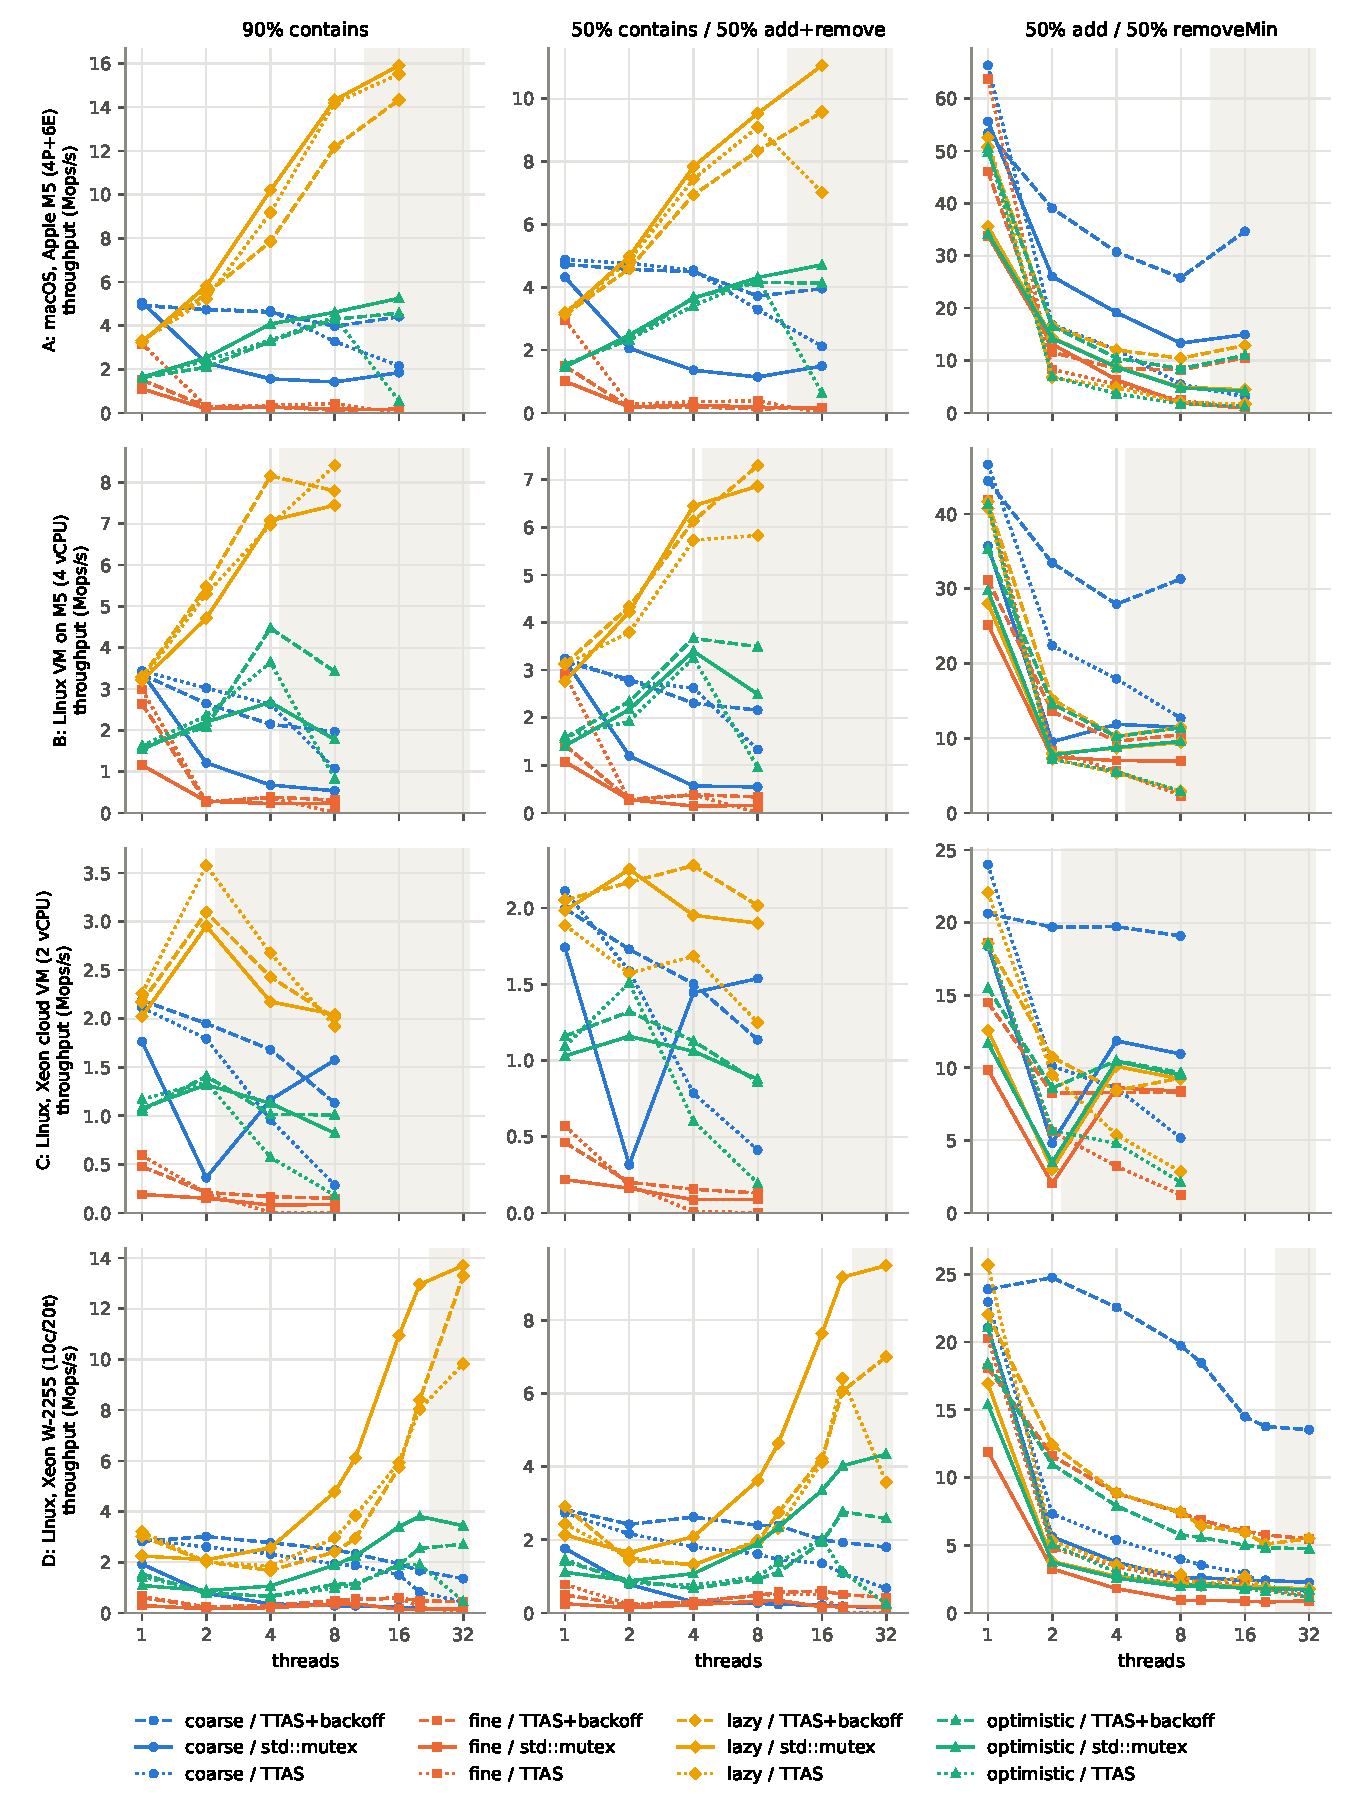
\includegraphics[width=\linewidth]{figures/fig5_clist.pdf}
\caption{Part 2: throughput of the 12 list/lock combinations on the four
platforms (rows) for the three workload mixes (columns). Median of 3 runs of
0.4\,s. Colour: list; line style: lock. The shaded region marks
oversubscription.}
\label{fig:clist}
\end{figure}

\begin{table}[H]
\centering
\scriptsize
\setlength{\tabcolsep}{4pt}
\caption{Part 2: throughput (million operations/s) for the read mix and the
priority-queue mix. TTAS rows are omitted (see Figure~\ref{fig:clist}).}
\label{tab:clist}
\begin{tabular}{lrrrrrrrrrrrr}
\toprule
 & \multicolumn{6}{c}{90\% \texttt{contains} (threads)} & \multicolumn{6}{c}{\texttt{add}/\texttt{removeMin} (threads)} \\
\cmidrule(lr){2-7}\cmidrule(lr){8-13}
List / lock & 1 & 2 & 4 & 8 & 16 & 32 & 1 & 2 & 4 & 8 & 16 & 32 \\
\midrule
\multicolumn{13}{l}{\emph{Platform A (macOS, Apple M5)}} \\
Coarse, \texttt{std::mutex} & 5.1 & 2.3 & 1.6 & 1.4 & 1.8 & -- & 55.6 & 26.0 & 19.2 & 13.3 & 14.9 & -- \\
Coarse, TTAS+backoff & 4.9 & 4.7 & 4.6 & 4.0 & 4.4 & -- & 53.4 & 39.1 & 30.7 & 25.8 & 34.7 & -- \\
Fine-grained, \texttt{std::mutex} & 1.1 & 0.2 & 0.3 & 0.2 & 0.2 & -- & 33.8 & 13.1 & 6.3 & 2.0 & 0.9 & -- \\
Fine-grained, TTAS+backoff & 1.5 & 0.3 & 0.3 & 0.1 & 0.2 & -- & 46.1 & 11.6 & 8.5 & 8.2 & 10.5 & -- \\
Optimistic, \texttt{std::mutex} & 1.6 & 2.5 & 4.1 & 4.6 & 5.2 & -- & 34.2 & 14.2 & 8.7 & 4.8 & 4.1 & -- \\
Optimistic, TTAS+backoff & 1.6 & 2.1 & 3.3 & 4.3 & 4.6 & -- & 49.8 & 16.6 & 10.5 & 8.4 & 11.0 & -- \\
Lazy, \texttt{std::mutex} & 3.2 & 5.8 & 10.2 & 14.3 & 15.9 & -- & 35.5 & 14.4 & 8.8 & 4.9 & 4.4 & -- \\
Lazy, TTAS+backoff & 3.3 & 5.5 & 7.8 & 12.2 & 14.3 & -- & 50.8 & 16.6 & 12.0 & 10.4 & 12.9 & -- \\
\midrule
\multicolumn{13}{l}{\emph{Platform B (Linux VM, 4 vCPU)}} \\
Coarse, \texttt{std::mutex} & 3.4 & 1.2 & 0.7 & 0.5 & -- & -- & 35.7 & 9.5 & 11.9 & 11.5 & -- & -- \\
Coarse, TTAS+backoff & 3.4 & 2.6 & 2.1 & 2.0 & -- & -- & 44.4 & 33.5 & 27.9 & 31.3 & -- & -- \\
Fine-grained, \texttt{std::mutex} & 1.2 & 0.3 & 0.2 & 0.2 & -- & -- & 25.2 & 7.5 & 7.0 & 6.9 & -- & -- \\
Fine-grained, TTAS+backoff & 2.6 & 0.3 & 0.4 & 0.3 & -- & -- & 31.1 & 13.6 & 9.6 & 10.5 & -- & -- \\
Optimistic, \texttt{std::mutex} & 1.5 & 2.2 & 2.7 & 1.8 & -- & -- & 29.8 & 7.8 & 8.8 & 9.6 & -- & -- \\
Optimistic, TTAS+backoff & 1.6 & 2.1 & 4.5 & 3.4 & -- & -- & 35.3 & 14.6 & 10.2 & 11.4 & -- & -- \\
Lazy, \texttt{std::mutex} & 3.2 & 4.7 & 7.1 & 7.4 & -- & -- & 28.0 & 7.9 & 8.7 & 9.4 & -- & -- \\
Lazy, TTAS+backoff & 3.3 & 5.5 & 8.2 & 7.8 & -- & -- & 41.7 & 15.2 & 10.3 & 11.5 & -- & -- \\
\midrule
\multicolumn{13}{l}{\emph{Platform C (Linux, Xeon, 2 vCPU)}} \\
Coarse, \texttt{std::mutex} & 1.8 & 0.4 & 1.2 & 1.6 & -- & -- & 18.4 & 4.8 & 11.9 & 11.0 & -- & -- \\
Coarse, TTAS+backoff & 2.2 & 1.9 & 1.7 & 1.1 & -- & -- & 20.6 & 19.7 & 19.7 & 19.1 & -- & -- \\
Fine-grained, \texttt{std::mutex} & 0.2 & 0.2 & 0.1 & 0.1 & -- & -- & 9.9 & 2.0 & 8.6 & 8.4 & -- & -- \\
Fine-grained, TTAS+backoff & 0.5 & 0.2 & 0.2 & 0.1 & -- & -- & 14.5 & 8.3 & 8.3 & 8.3 & -- & -- \\
Optimistic, \texttt{std::mutex} & 1.1 & 1.3 & 1.1 & 0.8 & -- & -- & 11.7 & 3.5 & 10.5 & 9.5 & -- & -- \\
Optimistic, TTAS+backoff & 1.1 & 1.4 & 1.0 & 1.0 & -- & -- & 15.5 & 8.6 & 10.5 & 9.7 & -- & -- \\
Lazy, \texttt{std::mutex} & 2.0 & 3.0 & 2.2 & 2.0 & -- & -- & 12.6 & 3.0 & 10.1 & 9.2 & -- & -- \\
Lazy, TTAS+backoff & 2.2 & 3.1 & 2.4 & 2.0 & -- & -- & 18.6 & 10.7 & 8.4 & 9.3 & -- & -- \\
\midrule
\multicolumn{13}{l}{\emph{Platform D (Linux, Xeon W-2255, 10c/20t)}} \\
Coarse, \texttt{std::mutex} & 1.9 & 0.8 & 0.4 & 0.3 & 0.2 & 0.1 & 21.1 & 5.6 & 3.7 & 2.5 & 2.4 & 2.3 \\
Coarse, TTAS+backoff & 2.8 & 3.0 & 2.8 & 2.5 & 1.9 & 1.4 & 23.9 & 24.8 & 22.6 & 19.7 & 14.5 & 13.5 \\
Fine-grained, \texttt{std::mutex} & 0.3 & 0.2 & 0.2 & 0.3 & 0.1 & 0.2 & 11.9 & 3.3 & 1.8 & 0.9 & 0.9 & 0.9 \\
Fine-grained, TTAS+backoff & 0.6 & 0.2 & 0.3 & 0.5 & 0.6 & 0.4 & 18.1 & 11.6 & 8.8 & 7.4 & 6.0 & 5.5 \\
Optimistic, \texttt{std::mutex} & 1.1 & 0.9 & 1.1 & 1.9 & 3.4 & 3.4 & 15.4 & 3.7 & 2.6 & 1.9 & 1.8 & 1.7 \\
Optimistic, TTAS+backoff & 1.5 & 0.8 & 0.7 & 1.1 & 1.9 & 2.7 & 18.4 & 11.0 & 7.9 & 5.8 & 5.0 & 4.7 \\
Lazy, \texttt{std::mutex} & 2.2 & 2.1 & 2.6 & 4.8 & 10.9 & 13.7 & 16.9 & 3.8 & 2.7 & 2.2 & 2.0 & 1.8 \\
Lazy, TTAS+backoff & 3.0 & 2.0 & 1.7 & 2.4 & 5.7 & 13.3 & 22.0 & 12.4 & 8.8 & 7.4 & 6.0 & 5.5 \\
\midrule
\multicolumn{13}{l}{\emph{Platform E (Windows, i5-9300H, 4c/8t)}} \\
Coarse, \texttt{std::mutex} & 2.5 & 1.1 & 0.9 & 0.8 & -- & -- & 11.4 & 6.6 & 4.6 & 5.1 & -- & -- \\
Coarse, TTAS+backoff & 2.0 & 1.9 & 1.7 & 1.4 & -- & -- & 8.4 & 8.3 & 6.4 & 5.0 & -- & -- \\
Fine-grained, \texttt{std::mutex} & 0.1 & 0.2 & 0.2 & 0.1 & -- & -- & 5.6 & 2.6 & 2.2 & 2.2 & -- & -- \\
Fine-grained, TTAS+backoff & 0.1 & 0.1 & 0.1 & 0.1 & -- & -- & 3.9 & 3.9 & 3.3 & 2.8 & -- & -- \\
Optimistic, \texttt{std::mutex} & 1.0 & 1.2 & 2.1 & 2.9 & -- & -- & 4.6 & 2.5 & 1.6 & 0.9 & -- & -- \\
Optimistic, TTAS+backoff & 1.0 & 1.0 & 1.1 & 1.6 & -- & -- & 3.7 & 3.0 & 2.5 & 2.0 & -- & -- \\
Lazy, \texttt{std::mutex} & 2.3 & 2.6 & 3.8 & 5.6 & -- & -- & 4.1 & 2.5 & 1.5 & 0.9 & -- & -- \\
Lazy, TTAS+backoff & 2.3 & 3.0 & 2.9 & 4.6 & -- & -- & 4.3 & 3.5 & 3.3 & 2.4 & -- & -- \\
\bottomrule
\end{tabular}

\end{table}

Figure~\ref{fig:clist} and Table~\ref{tab:clist} summarize the sweep.

\textbf{Only the lazy list scales.} With the read mix, the lazy list goes from
3.2 to 15.9\,Mops/s on Platform~A ($5\times$ at 16 threads), from 3.3 to
8.2\,Mops/s on Platform~B ($2.5\times$ at 4 threads), and to 13.7\,Mops/s on Platform~D (32 threads; 9.5\,Mops/s on \emph{update}). Its \texttt{contains}
takes no lock, and \texttt{add}/\texttt{remove} lock only two neighbouring
nodes after a lock-free search. The optimistic list scales less (1.6
$\rightarrow$ 4.6\,Mops/s on A) because its validation traverses the list a
second time. The coarse list cannot scale: with backoff it stays flat
(4.9 $\rightarrow$ 4.4\,Mops/s on A), and with \texttt{std::mutex} it degrades.

\textbf{The fine-grained list is the slowest.} A traversal of about 250 nodes
acquires and releases about 250 locks, and because threads cannot overtake
each other, the slowest thread sets the pace for all. Already at 2 threads it
falls to 0.3\,Mops/s or less on every platform (read mix).

\textbf{\texttt{removeMin} does not scale on any list.} In the priority-queue
mix every \texttt{removeMin} needs the same two nodes at the head of the list,
so the list behaves like one lock. Throughput drops as soon as a second thread
arrives (on A, 66 $\rightarrow$ 17\,Mops/s with TTAS on the coarse list) and
the variant with the cheapest critical section wins: the coarse list with
backoff, which loses least (53 $\rightarrow$ 26\,Mops/s at 8 threads on A,
and nearly flat at about 20\,Mops/s on C). This is the bottleneck that Part~3
inherits.

\textbf{Locks.} \texttt{std::mutex} collapses as soon as two threads contend on
Linux (coarse list, priority-queue mix on B: 35.7 $\rightarrow$
9.5\,Mops/s), because each contended hand-off puts a thread to sleep in the
kernel and wakes it up again. Pure TTAS collapses under oversubscription
(fine-grained list on A: 3.2 $\rightarrow$ 0.0\,Mops/s at 16 threads),
because waiting threads spin while the lock holder is descheduled. TTAS with
backoff is the best or nearly the best lock in almost every configuration. One
exception is the lazy list on macOS, where \texttt{std::mutex} is as good as
backoff (15.9 against 14.3\,Mops/s): the lazy list's locks are rarely
contended, and Apple's mutex spins briefly before it sleeps.
